\chapter{A hydrogen impurity measurement device for measuring ISO 14687 impurities}

\section*{Abstract}
In this chapter a device capable of performing hydrogen impurity enrichment is designed and tested under a number of conditions using a commercial membrane compared against the best performing fabricated membranes in chapter 5. 
Through the use of automation and optimisation of parameters the design of the enrichment device was improved to create a more efficient, safer, and user friendly device to meet the requirements of hydrogen impurty laboratories. PID temperature conrtol was implemented, allowing greater control of the heating rate and temperature within the enrichment device, preventing damage to the membrane which earlier designs were lacking. Temperature and pressure monitoring was also implemented and fed into a microcontroller which allows the operator to continuously monitor the process paraments, and calculated enrichment factor in real time. 

The improved hydrogen impurity enrichment device was then tested by performing enrichment on a number of synthetic hydrogen samples created using the procedure outlined in section \ref{exp-gasprep}, and a hydrogen sample taken from a hydrogen refuelling station. The device was capable of enriching samples to 50 times. Theoretically higher enrichment factors were possible but these tests were limited for safety reasons. The commercial membrane took 7 days to perform this measurement and provided the final value of within 2\% of the gravametrically calculated value using the tracer enrichment method which was deemed sufficient for a commercial device. The device was also tested using a sulphur containing sample which resulted in failure of all membranes. The PdCuZr membrane while identified as being a strong candidate for enriching sulphurous impurities, failed in all tests due to poor thermal stability of the support. The commercial membrane on the other hand reacted with the gases in the mixture and became completely inactive. \textcolor{red}{\textbf{HRS results pending}}


\section{Introduction}
Now that appropriate membrane compositions have been found, a number of improvements must be made to the hydrogen impurity enrichment device in order to make it suitable as a commercial process and product for measuerment of ISO 14687-2 impurities. All previous devices used were extremely manual and required close operator attention to ensure the experiment performed correctly. All enrichment factor calculations discussed in section \ref{exp-enrichproc} must also be calculated by hand, after the experiment has been performed, limiting the ability for the operator to plan the experiment in advance. In addition to this the krypton enrichment method which was identified as the best method for calculating the enrichment factor in section \ref{lit-enrichlit} but no procedure is in place to instruct operators on how to add this krypton to their sampling vessel. 

This chapter will provide a method for taking krypton spiked samples from a hydrogen refuelling station, improve the hydrogen impurity enrichment device through automation to improve the usability of the device, while providing real time results for the user, and quantify how the enrichment device performs when tested using a real sample froma  hydrogenr refuelling station. 

\section{Addition of krypton for tracer enrichment}\label{kryptonspike}
Past studies using tracer enrichment have simply added the krypton required when making a gas mixture through loop addition,\cite{Murugan2014} allowing for a known quantity of krypton to be added prior to any test. While this is appropriate when making a mixture from scratch, it is unsuitable for sampling from a hydrogen refuelling station, as the low pressure krypton cannot be added to a sample already taken. While there are some studies that have suceeded in adding low pressure gas to a high pressure sample using cryoegnics,\cite{Podesta2017} these tests were on a small scale and were deemed unsuitable for HRS sampling. The only avaliable option for spiking of the hydrogen samples was to add a known quantity of krypton to the already empty vessel, and analyse the final concentration of krypton afterwords to use in the enrichment factor calculations. The disadvantage of this method is that it adds an extra, higher uncertainty associated with the GC used to measure the krypton concentration. There are three variables which will effect the final krypton concentration added to the cylinder to alloy for tracer enrichment; the sampling vessel volume, the sample fill pressure from the hydrogen refuelling station, and the mass of krypton added.  

It is standard for hydrogen samples to be taken using a 10L vessel, although in the future operators may wish to take larger samples using a 50L cylinder, or smaller samples using a 1L cylinder. Although theoretically any sample size could be taken, these are generally the standard sample sizes used for metrology purposes and will be the only ones considered. The fill pressure of the sample has previously found to be unpredicable since it relies on sampling in line with a FCEV. Because of this, the final fill pressure of the sample cylinder be proportional to the amount of fuel remaining in the car. Despite this samples are generally not taken above 10 MPa for safety reasons. 

It was decided that the best procedure is to add a set mass of krypton to the desired sampling vessel prior to sampling taking place. The krypton is added to the evacuated sample cylinder using the procedure outlined in section \ref{exp-gasprep}. The sample can then be filled from the HRS using the procedure outlined in section \ref{exp-sampletake} and the mole fraction of krypton measured using the gas analysis procedure outlined in section \ref{exp-gasprep}. 16ENG01 MetroHyVe states that hydrogen samples should contain 1-10 \textmu mol/mol of krypton. Using the ideal gas law the mass of krypton required to ensure the krypton concentration stayed within these bounds was calculated. It was found that for samples below 10bar it was not possible to keep the concentration of krypton within the bounds of 1-10 \textmu mol/mol and therefore it is reccomended to ensure a sample higher than this is taken in order to ensure a reasonably high enrichment factor can be achieved during the subsequent experiments. The predicted concentrations of krypton compared to fill pressures at an assumed temperature of 20\textdegree C were calculated and shown in figure \ref{krsamples}. The results show that for a 1L cylinder 30.8 mg Kr should be added, for a 10L cylinder 300.79mg, and for a 50L cylinder 1484mg. This is enough to ensure concentrations between 1-10 \textmu mol/mol are achieved in pressures between 10-100 bar. 

\begin{figure}
    \centering
    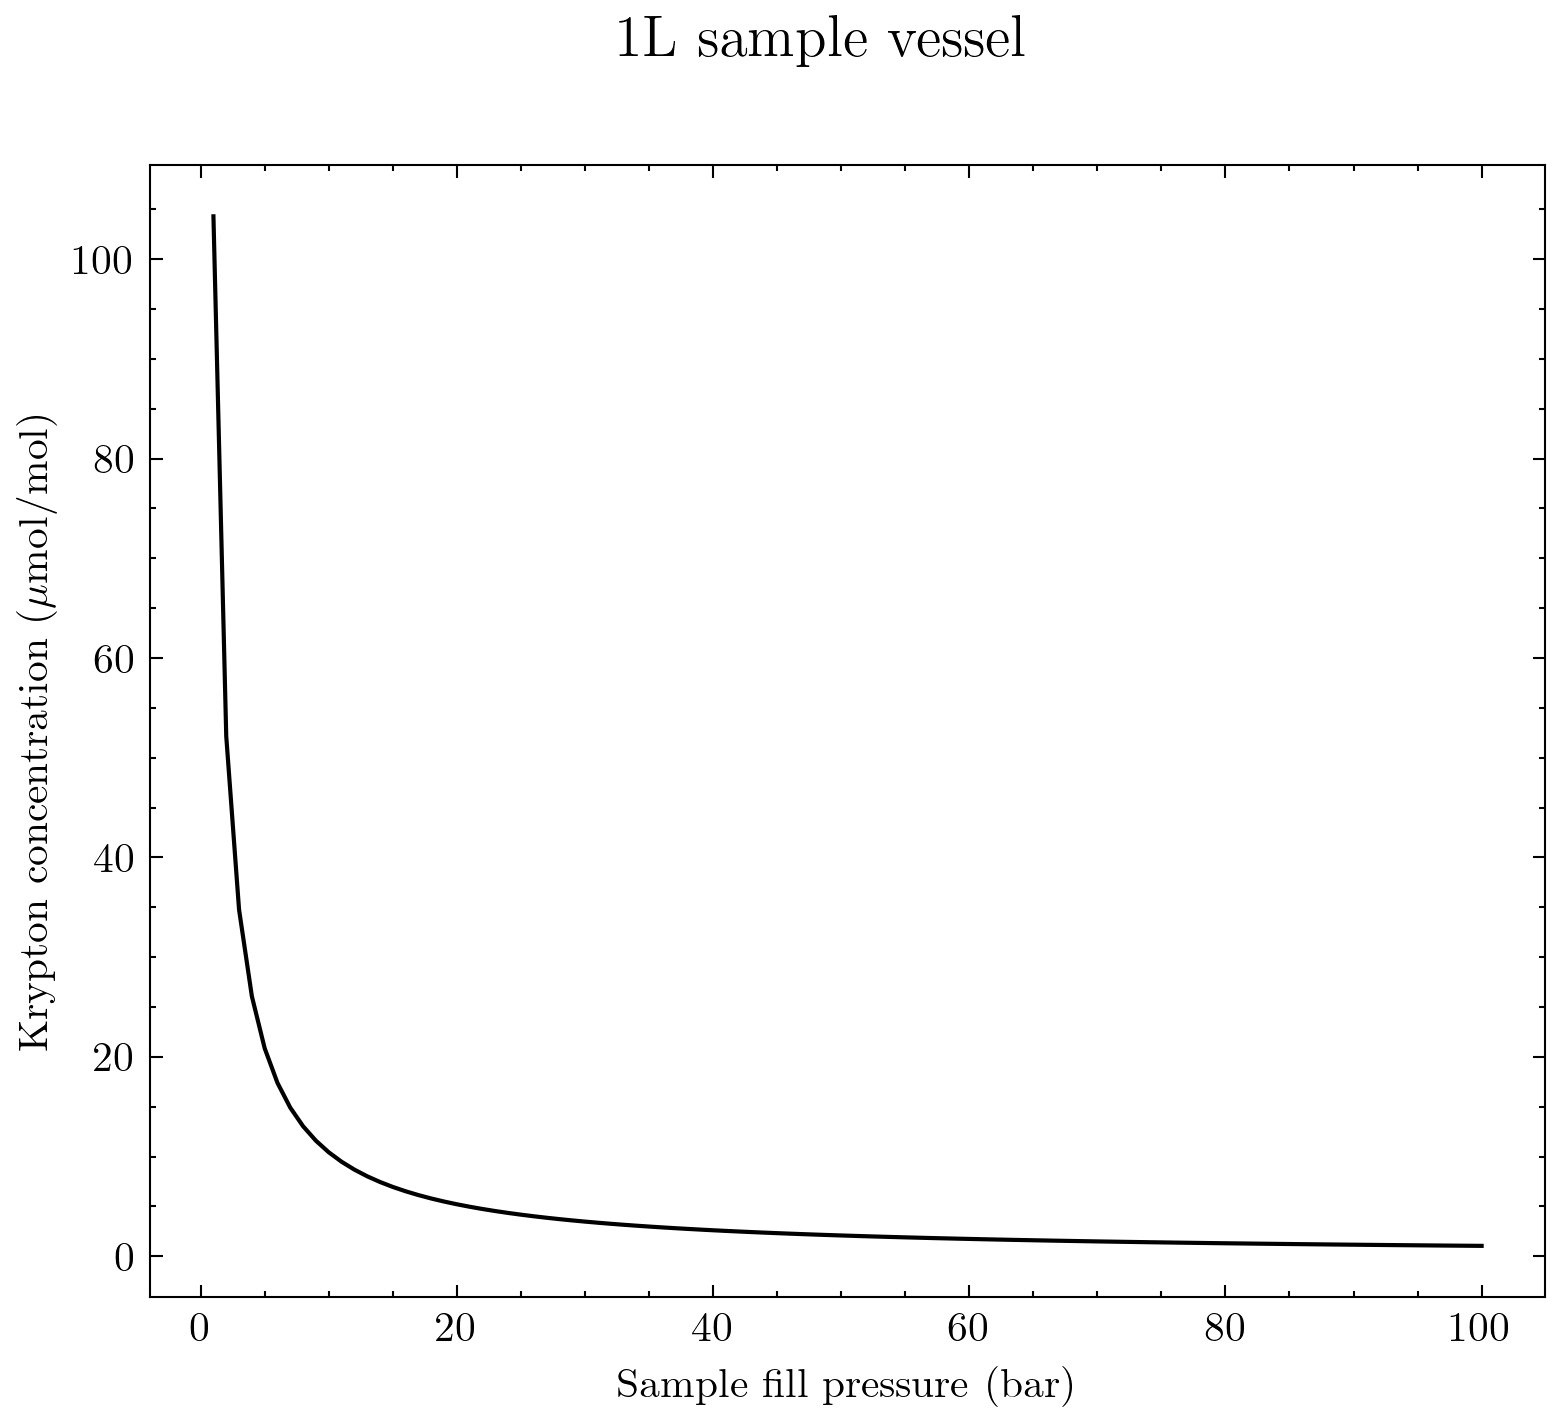
\includegraphics[width=0.5\linewidth, keepaspectratio]{/Users/marc/Thesis/Chapter5/1L.jpg}
    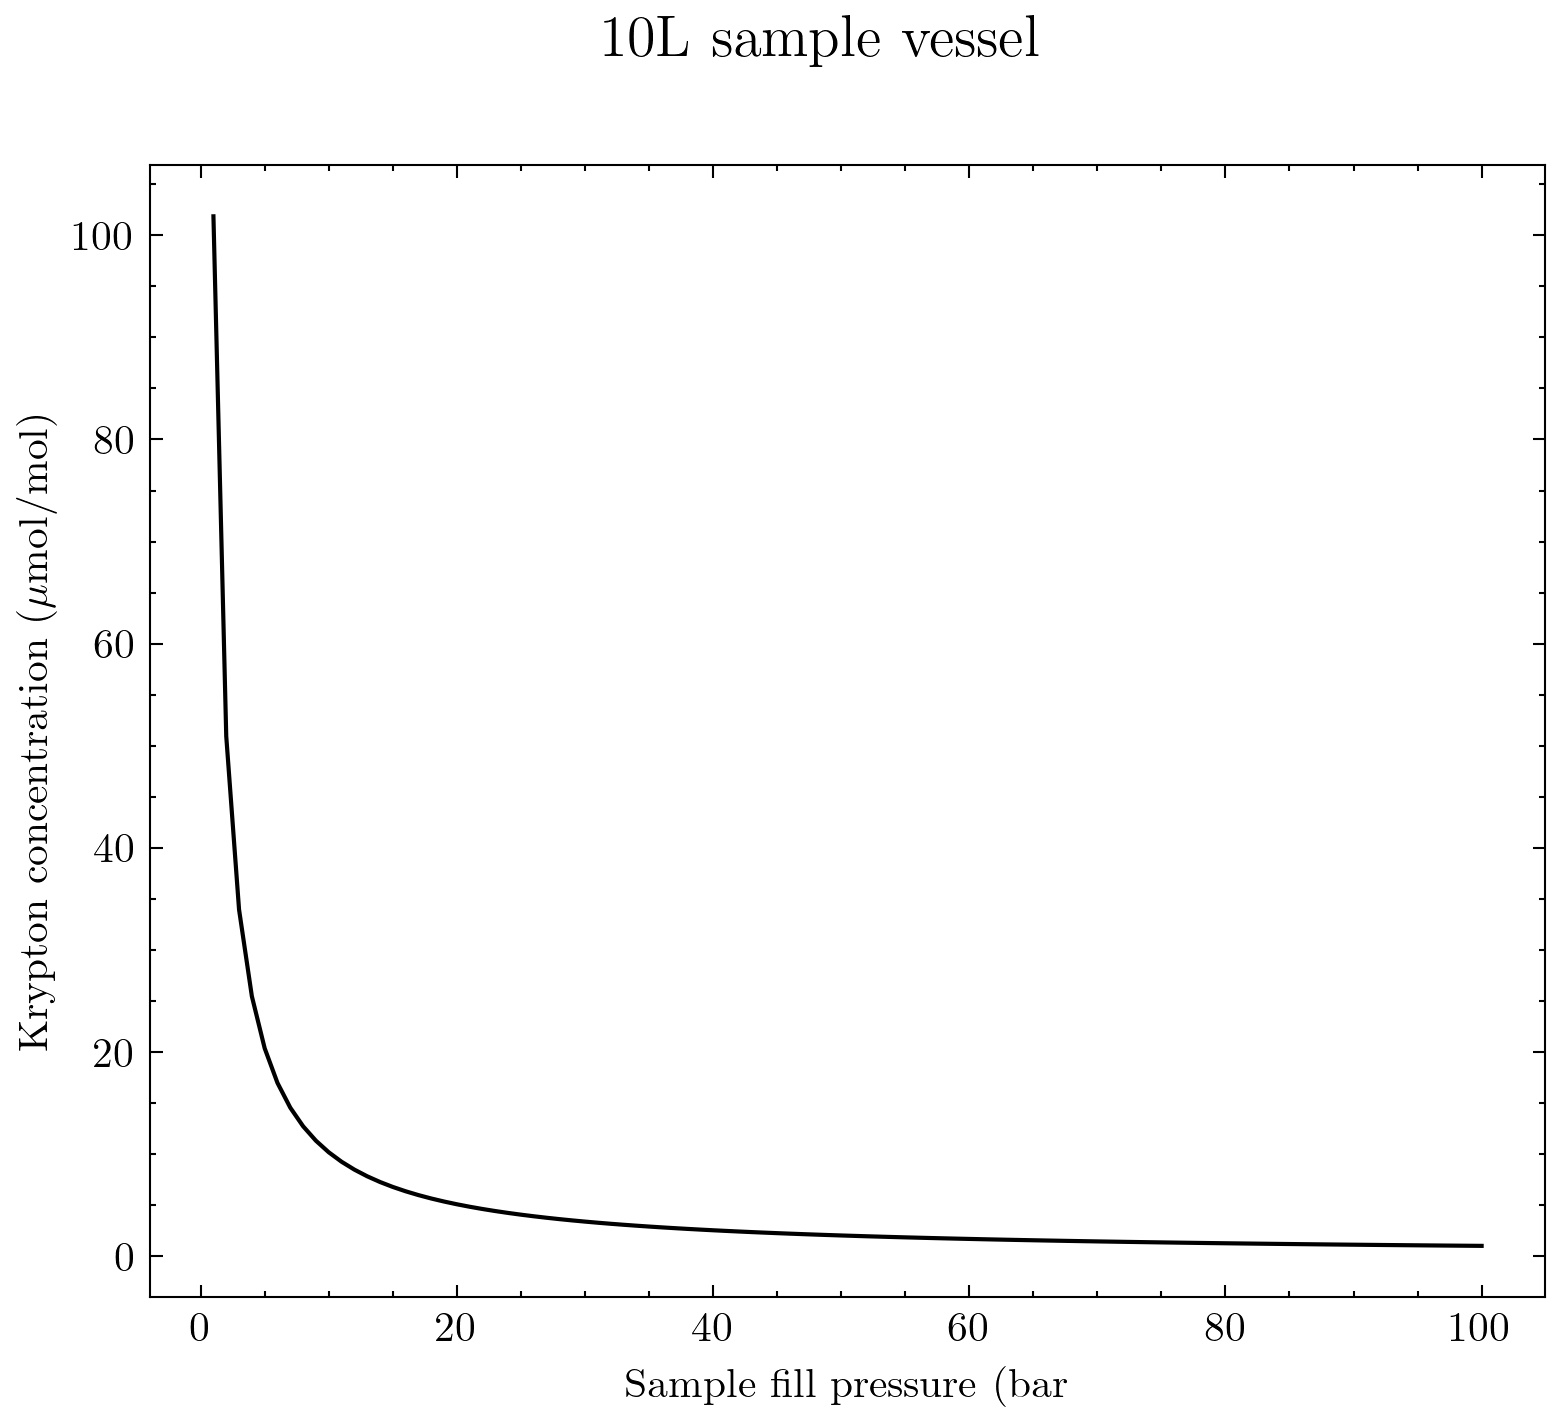
\includegraphics[width=0.5\linewidth, keepaspectratio]{/Users/marc/Thesis/Chapter5/10L.jpg}
    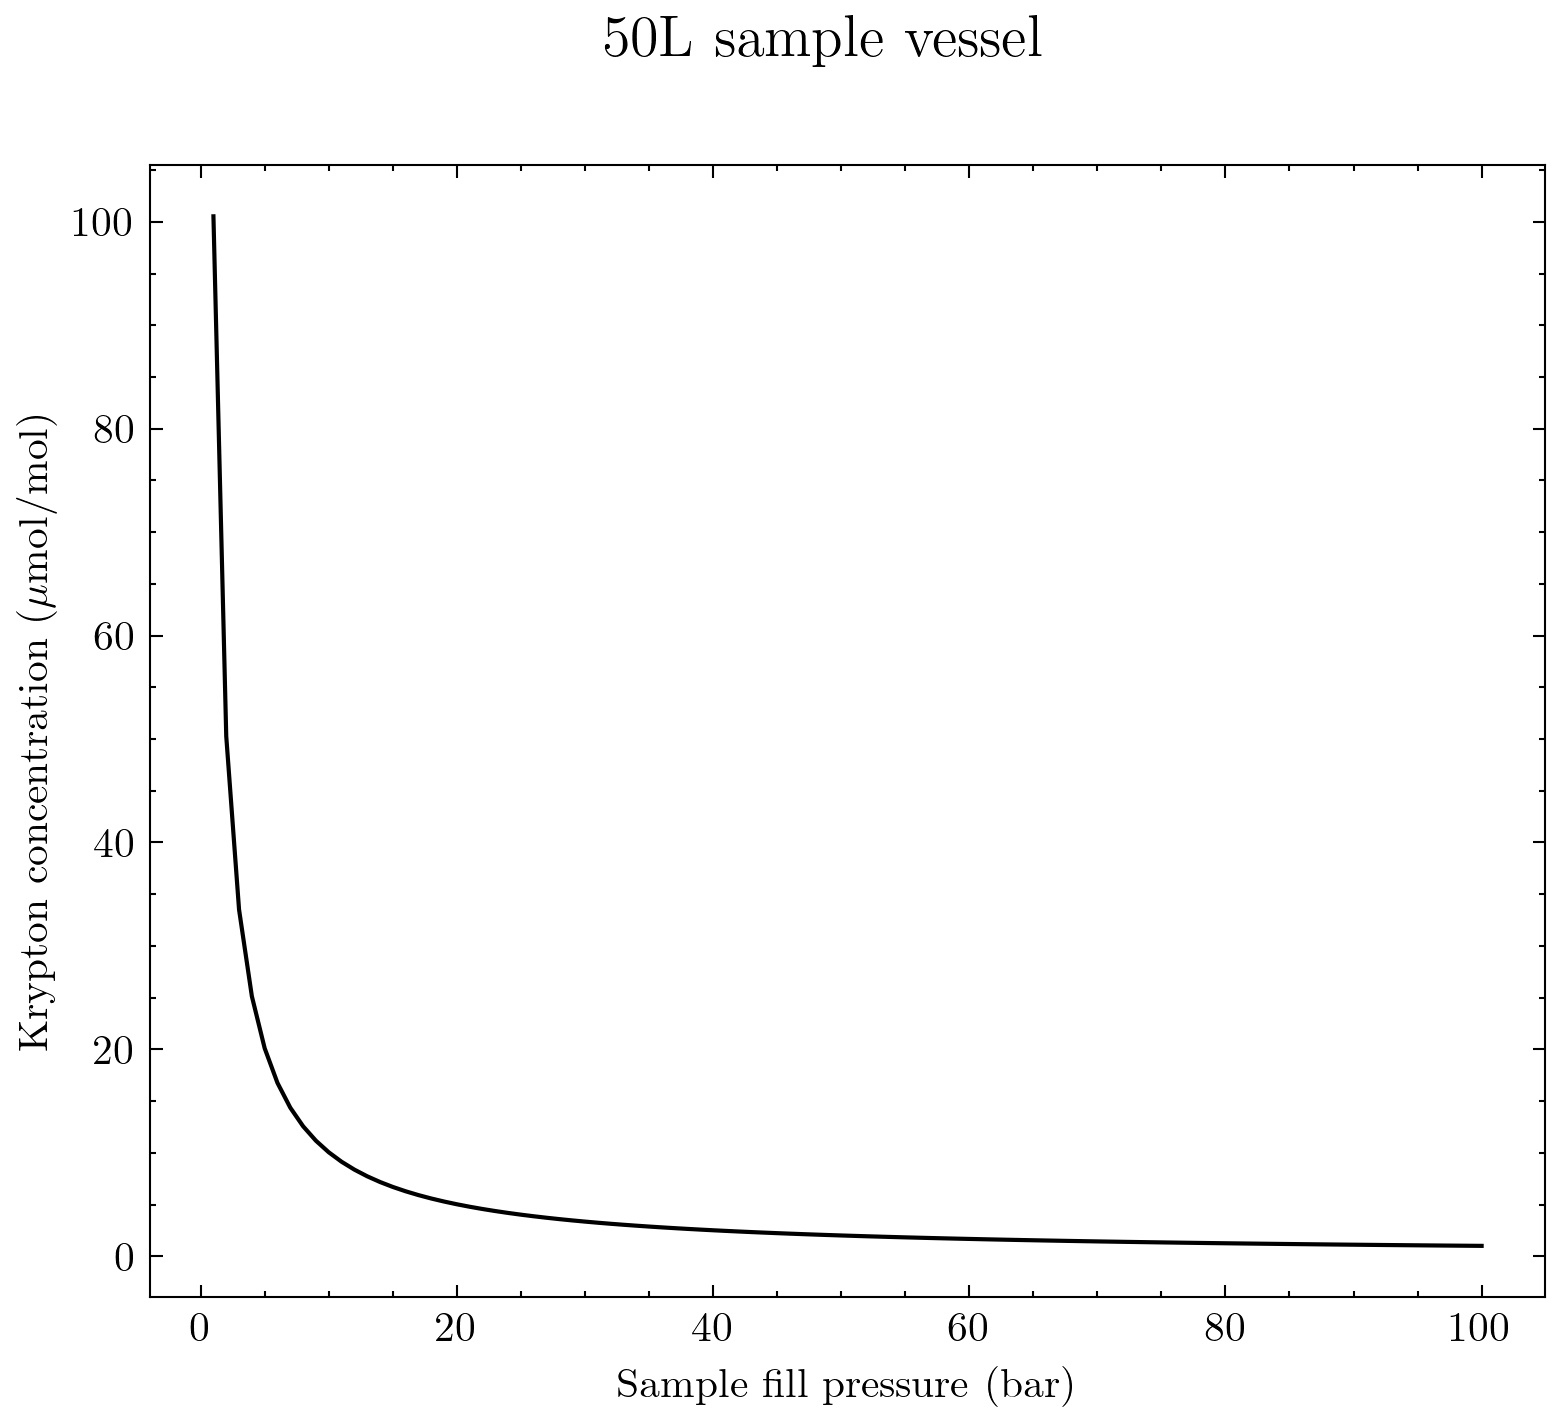
\includegraphics[width=0.5\linewidth, keepaspectratio]{/Users/marc/Thesis/Chapter5/50L.jpg}
    \caption{Predicted concentration of krypton within hydrogen samples in; 1L cylinder (30.8 mg Kr), 10L cylinder (300.79 mg Kr), 50L cylinder (1484 mg Kr)}
    \label{krsamples}
  \end{figure}

\section{Hydrogen Impurity enrichment device}
The aim of this section is to design an improved hydrogen impurity enrichment device which balances cost, accuracy and is operator-friendly. Automation will be taken into account in anticipation of the larger number of samples for analysis in the future and to improve the overall user experience. 
\subsection{Requirements}
Previous enrichment devices in literaure can be described as early prototypes.\cite{Ahmed2010} \cite{Murugan2014} In order to make the enrichment device commercially viable it must first be made more reliable. Greater control must be implemented over the pressures and temperatures within the device in order to ensure the membrane is not damaged inadvertently. Since the enrichment device operates by heating hydrogen to 300\textdegree C, adequate safety is of high concern. Previous enrichment devices in literature were lab scale, with the only safetry measures in place being those in the lab. Further safety and interlocks must be added to the enrichment device to ensure in the event of equipment failure the system can shut down safety. Finally all past devices involved the user manually recording important process values by hand, which is unintuitive, susceptible to errors, and does not allow easy monitoring system. An intuitive interface between the operator and the system will be added in order to automatically calculate output values such as the CEF, delivering this to the operator along with other important process parameters. 

\begin{itemize}
    \item Improve reliability by providing greater control over process parameters
    \item Improve safety by adding additional interlocks
    \item Improve user experience through in-situ process monitoring and data analysis
\end{itemize}

\subsection{System design}
The redesigned HIED is shown in figure \ref{hiedpid}. All tubing and pressure fittings were supplied by Swagelok \cite{swagelok} and the system was manufactured by Strata Technology London. \cite{stratatechnology}

The system is split into two units, the stationary unit and the transportable unit. The stationary unit is the bulk of the system, and contains piping to transport the gases to the enrichment device, connections for two gas cylinders for nitrogen (Q1) and the hydrogen sample to be tested (Q2), pressure relief valves (PSV001 \& PSV002), and connections to the vaccum system and gas vents. 

The transportable unit contains the enrichment vessel, heating and temperature control equipment, and the membrane. The enrichment vessel is a 300 cm\textsuperscript{3} sulfinert \cite{sulfinerttreatedsamplecylinder} treated vessel. The membrane is connected to one end of the vessel and operates in dead end mode. 

\subsubsection*{Safety}
It was decided that a nitrogen cylinder should be added to the system in order to ensure safety. Prior to evacuating the enrichment device the system should be purged 7 times with nitrogen  as this is adequate to reduce the concentration of gases remaining in the vessel, in particular the oxygen in air and any leftover hydrogen from previous tests, to a low enough level where it is not dangerous. \cite{BACQUART20205565} The enrichment device must be evacuated to a high vacuum before testing in order to ensure integrity of the results. Many commercially avaliable vacuum systems are not safe for use in explosive environments, therefore purging with nitrogen is a requirement before any procedures are to take place in the system. 

There are two pressure relief valves on the system. PSV001 is the safety interlock in the stationary unit and is set at 103 bar bar ensuring that in the event a higher pressure cylinder is connected to the system, there are sufficient safety measures in place. PSV002 is the pressure relief valve for the transportable unit, although is only in operation when it is connected to the stationary unit. and is set to 25 bar in order to prevent overpressurisation of the membrane. This pressure relief valve is critical when operating the enrichment device as the pressure initially in the enrichment vessel is at ambient temperature. As the enrichment vessel heats to the desired operating temperature, this pressure will increase, and since the enrichment vessel operates in dead end mode it is the only way out the system. This will cause the pressure within the enrichment vessel to potentially increase above the temperature rating of the membrane, resulting in failure. The pressure within the enrichment vessel is set using pressure controller PC001, effectivley creating two safety interlocks for the enrichment vessel. In the event of a pressure relief valve being triggered the gas will be automatically purged from the system through the vent.

\begin{landscape}
\begin{figure}
    \centering
    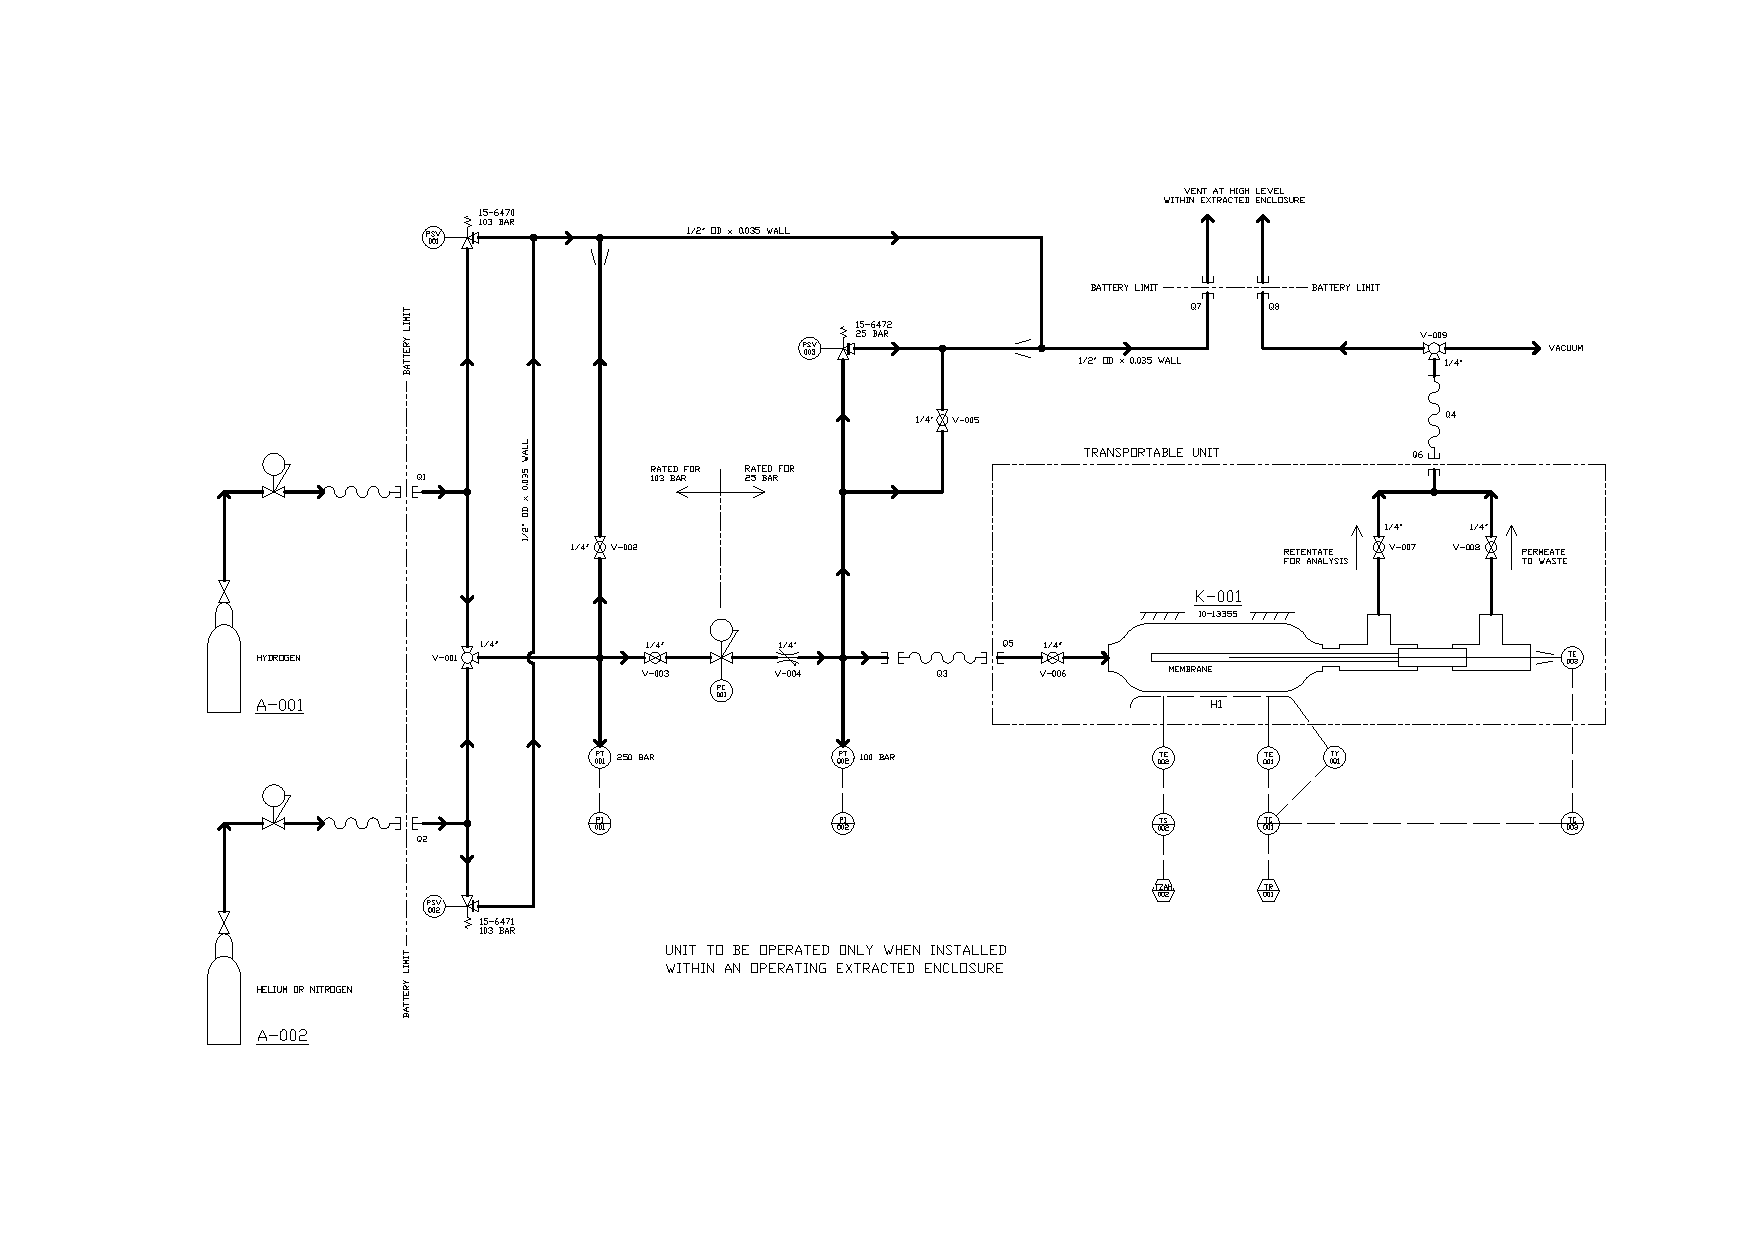
\includegraphics[height=0.5\pdfpageheight, keepaspectratio]{/Users/marc/Thesis/Chapter5/PID.pdf}
    \caption{P\&ID for the redesigned hydrogen impurity enrichment device}
    \label{hiedpid}
\end{figure}
\end{landscape}

\subsubsection*{User experience}
The main improvement to the user experience is through the segmentation of the system into the stationary unit and transportable unit which is shown in figure \ref{TU}. Bench space in a lab is often limited so often it is often not always possible to place the enrichment device next to the analyser that will be used following enrichment. Previous iterations of the enrichment device required either transporting the whole device, which is a difficult and potentially dangerous task, or disconnecting the swagelok fittings and transporting the vessel this way. While swagelok fittings can technically be disconected and reconnected, it is not reccomended since they are designed to be permenent pressure fittings, and the more times this operation is repeated, the faster components will have to be replaced. 

The transportable unit replaces these with VCR fittings, which are designed for disconnection and reconnection. The transportable unit also contains connections for the thermocouples connected to the temperature monitoring and control system, and the electrican connection to the system which are all designed for easy removal and reconnection. Finally the ergonomics of transporting the device have been improved through addition of a handle, allowing for eary transportation without unintentionally placing any strain on the pressure fittings. 
\begin{figure}
    \centering
    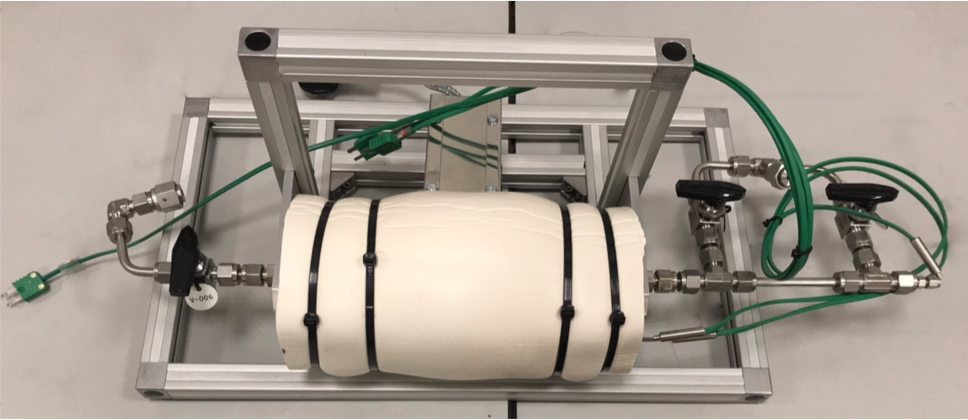
\includegraphics[width=\linewidth, keepaspectratio]{/Users/marc/Thesis/figures/TU.png}
    \caption{Disconnected transportable unit}
    \label{TU}
\end{figure}

\subsubsection*{Reliability}
The main improvement in reliability is a result of less instances of breaking and reconnecting fittings. As the system has been split into the stationary unit and transportable unit, the pressure fittings will gain an increased lifespan. Since the system is stationary it can benefit from being permenently connected to an evacuation rig and nitrogen supply. In the event of leakage multiple valves are implemented to allow the user to isolate different parts of the system in order to identify and replace the leaking component.

\subsection{Control/Measurement system}
There are two main factors to control for the enrichment device, the temperature and pressure. In past iterations of these systems control and measurement was done manually and hardwired into the system. By implementing adequate systems to measure and control these values operation of the system becomes easier, safer and more reliable 

The temperature of the enrichment vessel is changed using heating tape wrapped around the heating tape, and then covered in several layers of insulation. Pressure is controlled using a tamper proof temperature controller.  

\subsubsection*{Reliability}
The original system used an On/Off temperature controller, which simply measured the temperature using a thermocouple placed inside the membrane (TE003, figure \ref{hiedpid}), when the temperature rises above the setpoint the heater is switched off, when it drops below the heater is switched back on. The solution was unreliable, for example when the temperature setpoint was set at 300\textdegree C, the average value recorded was 302.7\textdegree C, with a standard deviation of 5\textdegree C. This is shown in figure \ref{TCcompare}. 

The system was upgraded with a PID temperature controller (OMRON), which continuously calculates an error value as the difference between a desired setpoint (SP) and a measured process variable (PV) and applies a correction based on proportional, integral, and derivative terms. This change in contro loop mechanism inproved the overall control of the system, bringing the average temperture recorded over 1 hour down to 302.7\textdegree C and the standard deviation down to 1.78\textdegree C.

\begin{figure}
    \centering
    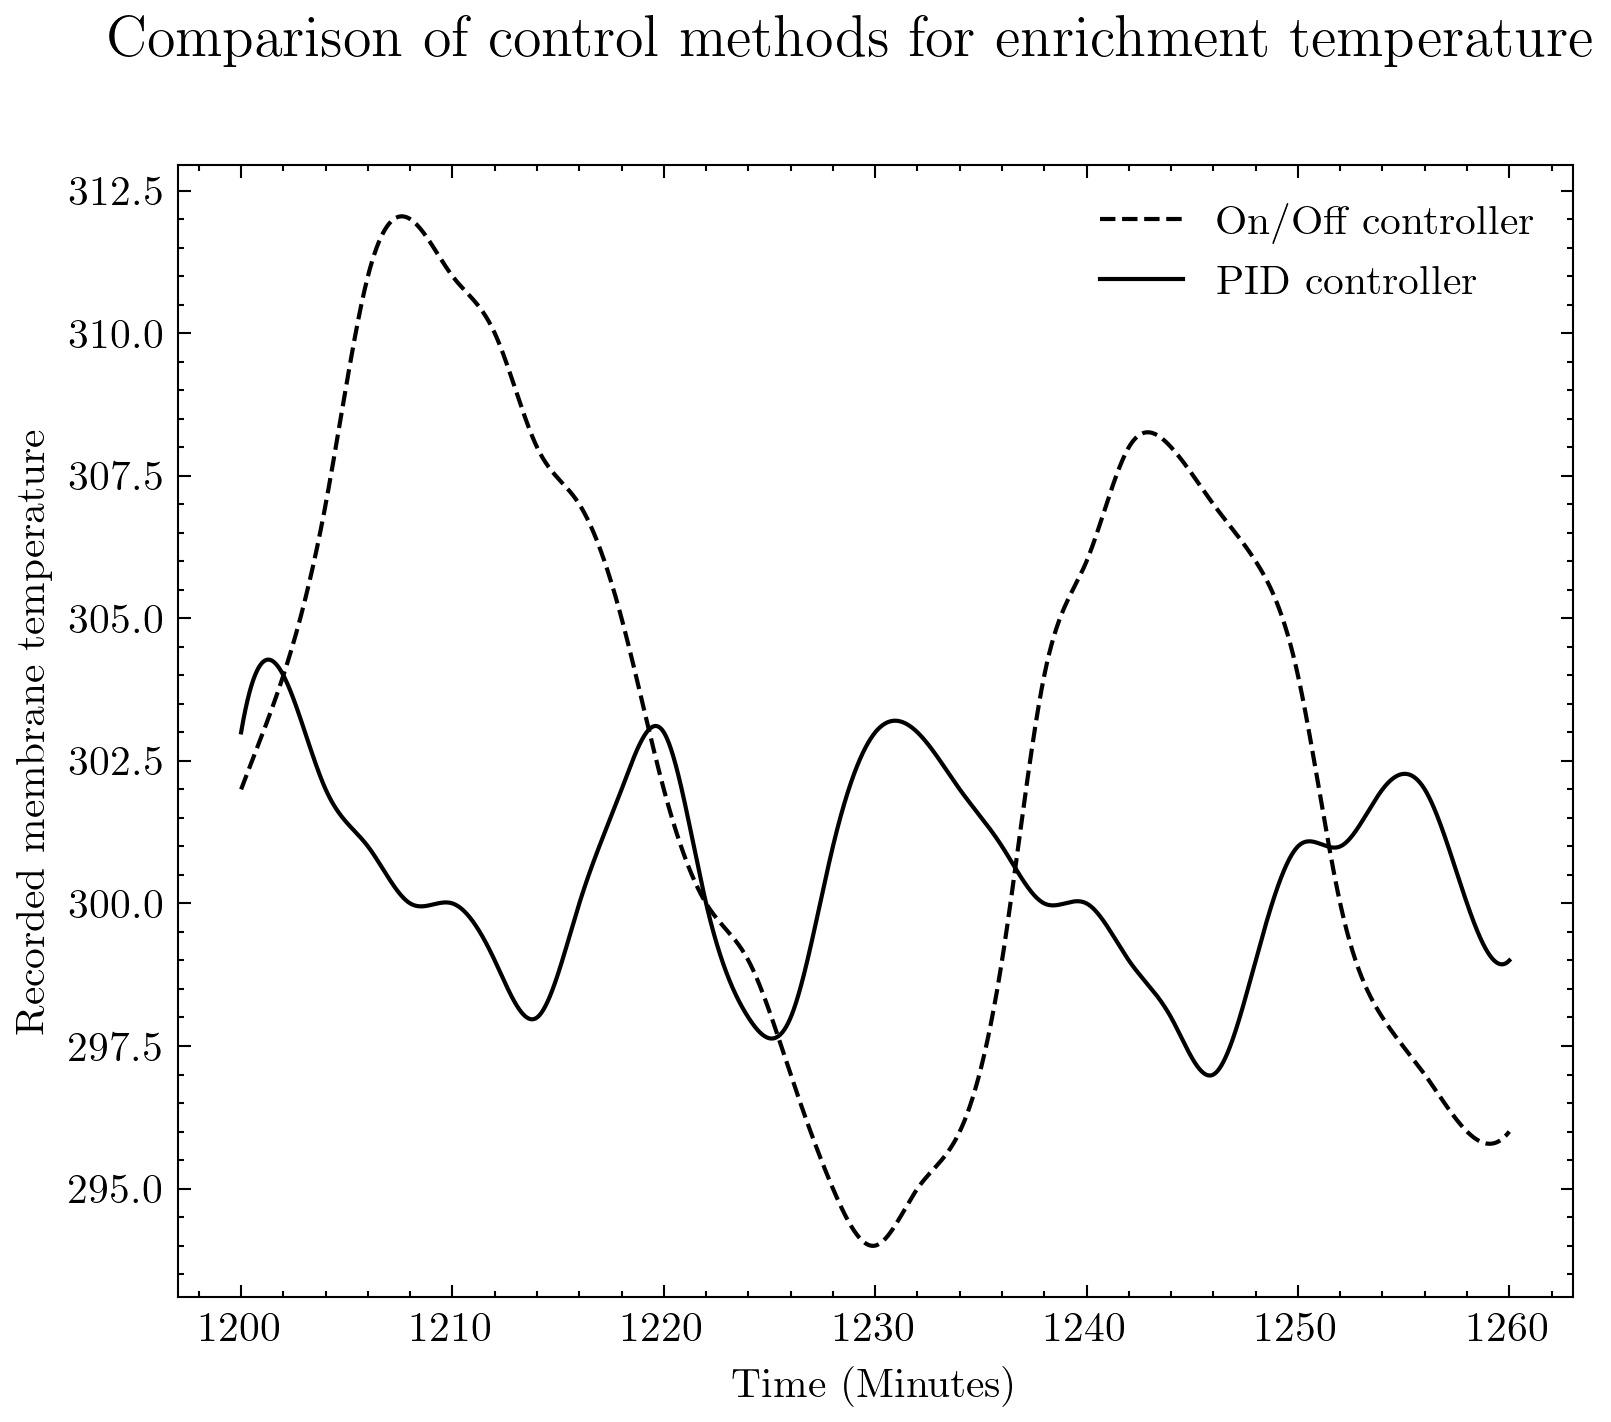
\includegraphics[width=\linewidth, keepaspectratio]{/Users/marc/Thesis/Chapter5/TC.jpg}
    \caption{Comparison of the On/Off temperature controller and PID temperature controller over a 1 hour period}
    \label{TCcompare}
\end{figure}

The pressure controller (PC001, figure \ref{hiedpid}) is considered reliable, as it can be set at a fixed pressure, which cannot be changed accidently by the user. The issue with reliability came from the measurement of pressure. Originally only one pressure sensor was used to measure the pressure inside the enrichment vessel (K-001), with the pressure of the sample cylinder used to calculate the enrichment factor only being measured once before and after the test. Two high resolution pressure sensors (Balluff) were added before and after the pressure controller so that both of these values could be monitored during the experiments. 

\subsubsection*{Safety}
The safety of the process was improved by adding a temperature shutoff to the enrichment vessel. There are three thermocouples (TE001, TE002 and TE003) on the enrichment vessel. TE003 is for controlling and monitoring the temperature of the membrane, while TE002 is for monitoring the temperature outside the vessell. TE003, which also measured the temperature outside the vessel, is connected to a temperature cut off, which is set 25\textdegree C above the setpoint temperature of the enrichment vessel. If the the recorded temperature outside of the enrichment vessel passes this threshold the heater will activate a trip, cutting off electricity until the device is checked by the operator. 

\subsubsection*{User experience}
The main improvement to user experience is the ability to easily control the temperature of the system. Previously the temperature controller was hardwired in, giving the user little control over the setpoint and temperature ramp of the device. With the new system these values can be controlled easily directly through the temperature controller, or using a microcontroller connected to the temperature controller, allowing more options for the operator.

\subsection{Data processing}\label{dataproc}
Data collection and processing was done manually and no automation was involved. The main improvement in the new system involved the use of a microcontroller to automatically log process variables. These values were stored for later processing by the user. A data analysis script was also prepared in order to estimate the time remaining for the experiment to reach the desired enrichment factor, and the current enrichment factor achieved. At the beginning of the experiment the user had the option of entering their desired enrichment factor. If entered this would be stored and the experiment would start. The system would then automatically log the initial pressures of the, hydrogen cylinder and enrichment vessel as $P_{1,a}$ and $P_{2,a}$, and the initial temperature of the enrichment vessel as $T_{1,a}$ and $T_{2,a}$ for the non ideal gas law enrichment factor (equation \ref{lit-eq:1}). The script would then continuously measure values for $P_{1,b}$, $P_{2,b}$, and $T_{2, b}$ and use them to calculate the current non-ideal gas law enrichment factor in real time. Note it was assumed the temperature of the sample cylinder ($T_{2,a}$) would remain constant at ambient temperature. This process is shown in pseudocode in figure \ref{pseudocode} and the user interface and GUI presented to the user can be found in the appendix. It should be noted that it was only possible to calculate the non-ideal gas law enrichment factor in real time as it is not possible to continuously monitor the concentration of the inert tracer molecule in the enrichment vessel. 

It has already been concluded in section \ref{lit-enrichlit} that the tracer enrichment method is the best method for calculating the enrichment factor and therefore this method will still be used going forward. Calculating the non-ideal gas law enrichment factor in this manner however acts as a useful safety measure to ensure the user has a rough estimate of what gas is within the vessel at any given time. It is also useful to store this information to identify when leaks have occured as discussed in section \ref{lit-enrichlit}.

\begin{figure}
    \centering
    
\includegraphics[width=\linewidth, keepaspectratio]{/Users/marc/Thesis/Chapter5/pseudocode.png}
    \caption{Diagrammatic representation of the data processing algorithm used to provide real time enrichment factor}
    \label{pseudocode}
\end{figure}

\section{Enrichment of hydrogen samples}
Enrichment of the hydrogen samples was performed using the set up shown in figure \ref{hiedpid}. An initial test was performed using a commercial membrane supplied by REB using an inert mixture created using the procedure in section \ref{exp-gasprep} in order to calculate the uncertainty associated with the device. Both the commercial and PdCuZr membrane identified as the best performing membrane in chapter 5 were tested using a synthetic gas mixture containing sulphur containing compounds, and krypton. Finally both the commercial membrane and PdCuZr membrane were tested using a sample taken from the hydrogen refuelling station using the procedure outlined in section \ref{exp-sampletake}.

In each case the system was purged 7 times with the hydrogen sample to ensure there was no air present in the system. Enrichment was performed at a temperature of 300\textdegree C and a final enrichment pressure of 5 bar. Enrichment factors were calculated using both the tracer enrichment method (equation \ref{lit-eq:2}) calculated at the end of the test, and non-ideal gas law method (\ref{lit-eq:2}) calculated using the data processing script described in section \ref{dataproc}.

The gas mixtures used in the inert and sulphur tests are shown in table \ref{inert} and \ref{exp-sulf}. Prior to testing the HRS sample was tested to verify the concentration of krypton, and ensure there was no oxygen present in the system to pose as a hazard. Enrichment factors were capped at 100 to ensure any residual oxygen would not reach a high enough concentration to create an explosive environment.

\begin{table}[]
    \centering
    \caption{Gas mixture composition of the inert sample used during enrichment tests}
    \label{inert}
    \begin{tabular}{@{}cc@{}}
    \toprule
    Impurity & \begin{tabular}[c]{@{}c@{}}Concentration \\ ($\mu$mol/mol)\end{tabular} \\ \midrule
    N\textsubscript{2}       & 6.598                                                               \\
    Kr       & 5.984                                                               \\
    H\textsubscript{2}       & Balance                                                             \\ \bottomrule
    \end{tabular}
    \end{table}

\subsection{Inert components}\label{inertsec}
The inert mixture in table \ref{inert} was enriched to a CEF value of 50. The enrichment period was performed over a 7 day period due to the low flux value achieved by the commercial membrane supplied. The $CEF_{NI}$ value was calculated using the algorithm decscibed in section \ref{dataproc} and can it's progress over the 7 day period shown in figure \ref{GCNI}. The $CEF_{NI}$ slightly overshot the desired value of 50, stabilising at a value of 54.33, and as can be seen varied widely over the course of the experiment due to signal noise and interference. The value is still useful for keeping track of the progress of the experiment. 

The system was not operated continuously for 180 hours, and was switched off at night when monitoring was not possible. This is why the $CEF_{NI}$ value fluctuated over time. 

\begin{landscape}
    \begin{figure}
        \centering
        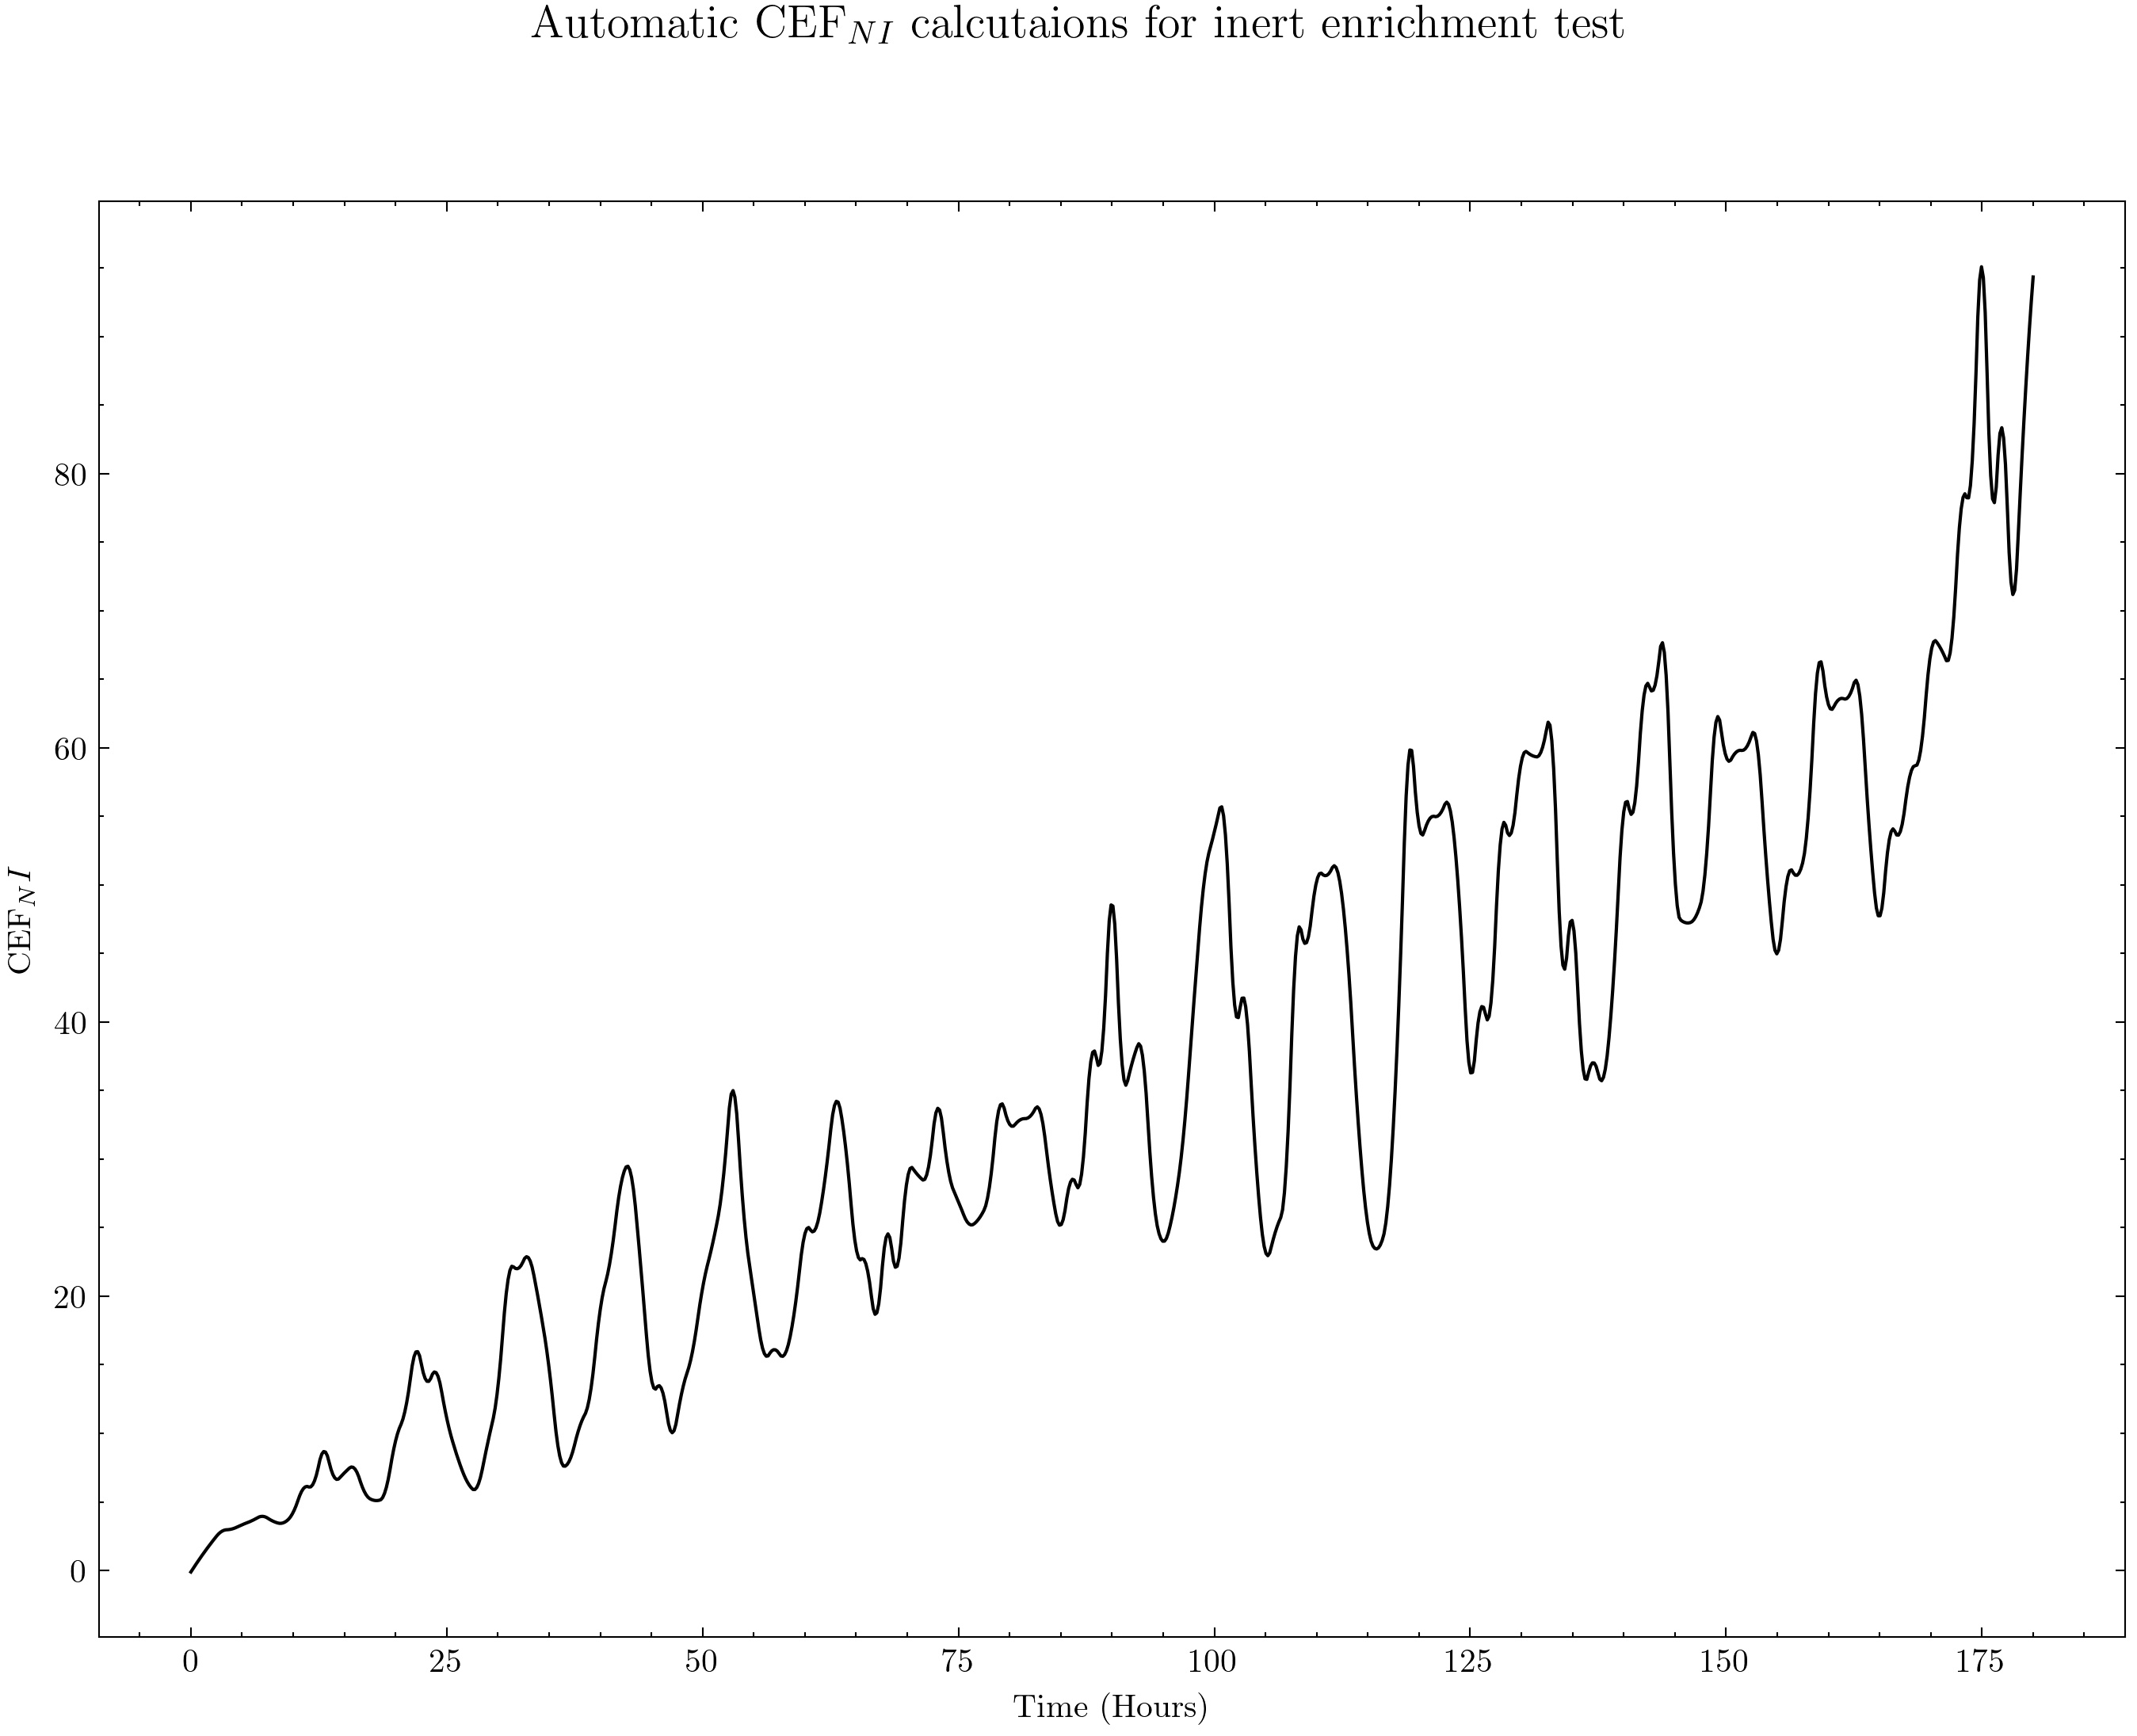
\includegraphics[width=0.9\linewidth, keepaspectratio]{/Users/marc/Thesis/Chapter5/inertenrich.jpg}
        \caption{$CEF_{NI}$ over the 180 hour enrichment of the inert hydrogen sample shown in table \ref{inert}}
        \label{GCNI}
    \end{figure}
\end{landscape}

Once the enrichment was complete, the system was isolated and left to cool. The transportable unit was then disconnected and it's composition measured and compared with it's original composition. Results were compared to nitrogen samples containing 251 nmol/mol, 500.77 nmol/mol, 1064 nmol/mol, 1437.37 nmol/mol using a derived calibration curve to account for non-linearity of the detector. The GC-PDHID data is shown in figure \ref{GCinert}. This anslysis found that the enriched gas contained 306.92 \textmu mol/mol of krypton and 332.14 \textmu mol/mol of Nitrogen. Calculating the $CEF_T$ using the tracer enrichment method gave a value of 51.23. 

The calculation using $CEF_{NI}$ gave an initial Nitrogen concentration of 6.11 \textmu mol/mol (-7\%)N\textsubscript{2}. The tracer enrichment method calculated a value of 6.48 \textmu mol/mol (-1.7\%) further showing that the tracer enrichment method provides a more accurate result. 

\begin{figure}[H]
    \centering
    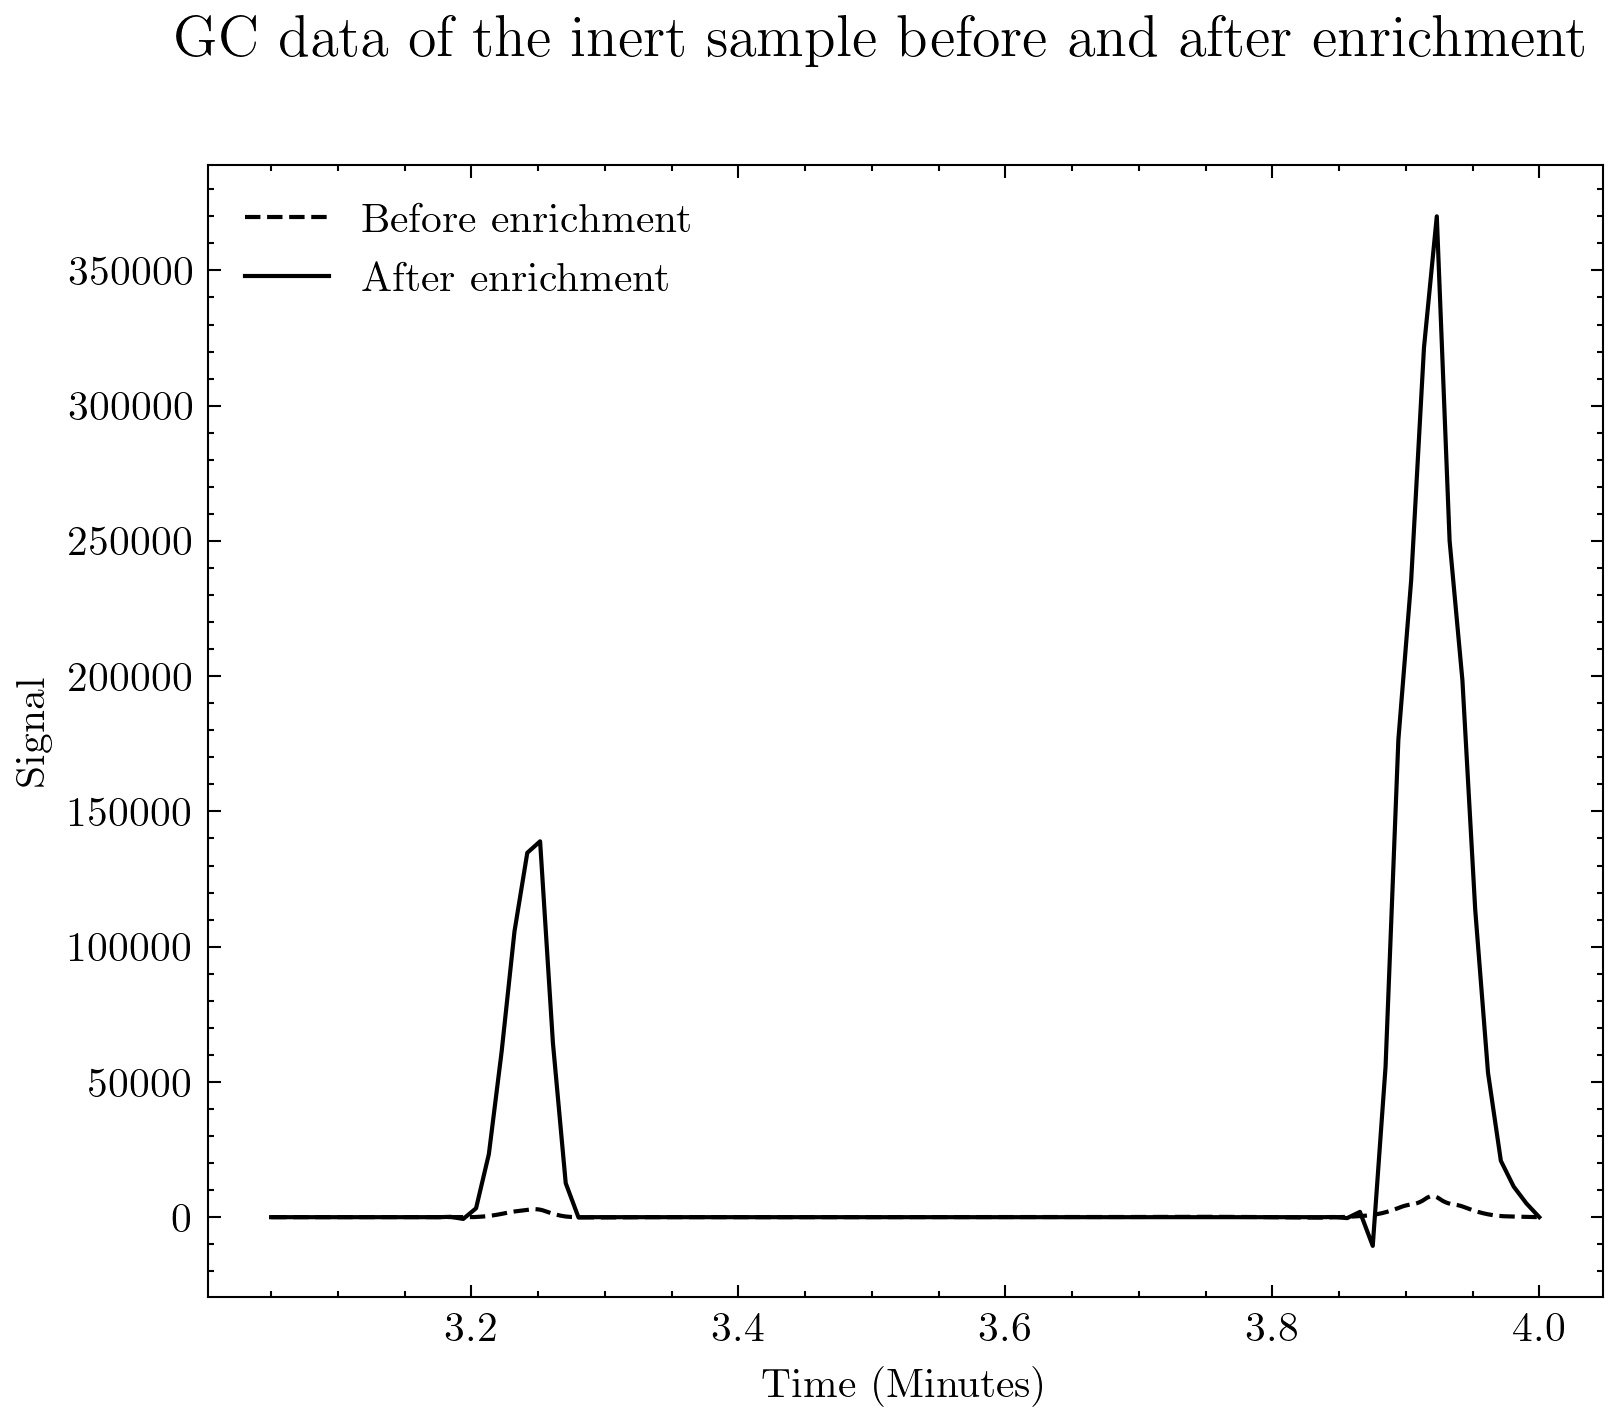
\includegraphics[width=\linewidth, keepaspectratio]{/Users/marc/Thesis/Chapter5/inertgc.jpg}
    \caption{GC-PDHID data of the inert sample both before and after enrichment with N\textsubscript{2} peaks shown at Time=3.25, and Kr peaks shown at Time=3.92}
    \label{GCinert}
\end{figure}

\subsection{Sulphur containing compounds}
The sulphur containing samples were tested using the same set up as section \ref{inertsec}, with the commercial PdAgAu membrane, and the PdCuZr alloy manufactured in chapter \label{proc-testingchapref}. The $CEF_{NI}$ values calculated in line for the experiment are shown in figure \ref{GCSULF}.

The commercial membrane saw the same dramatic drop in permeability as observed in chapter \ref{proc-testingchapref}. The experiment continued however it became clear that the permeability of the commercial membrane was dropping as the experiment went on, eventually becoming inactive to hydrogen permeability. The experiment was stopped. Upon analysis of the gas remaining within the enrichment vessel it was noted that the composition had significantly changed. This is shown in figure \ref{GCSULFCOMM}. The OCS, t-BuSH, THT and CS\textsubscript{2} in the gas mixture had reacted with the hydrogen to form H\textsubscript{2}S. While this would not effect the results of analysis much, sine the ISO 14687-2 standard does not give a maximum level of a specific sulphur containing compound, only the total concentration, OCS, THT, T-BuSH and CS\textsubscript{2} all contain carbon molecules. The result of this could be the formation of hydrocarbons, CO, or solid carbon on the surface of the membrane. In the case of carbon deposition, this would explain the complete deactivation of the membrane as discussed previously in section \ref{lit-pdreview}. In order to prevent this the exact reactions should be determined and process parameters further optimised to inhibit them from taking place. 

\begin{figure}[H]
    \centering
    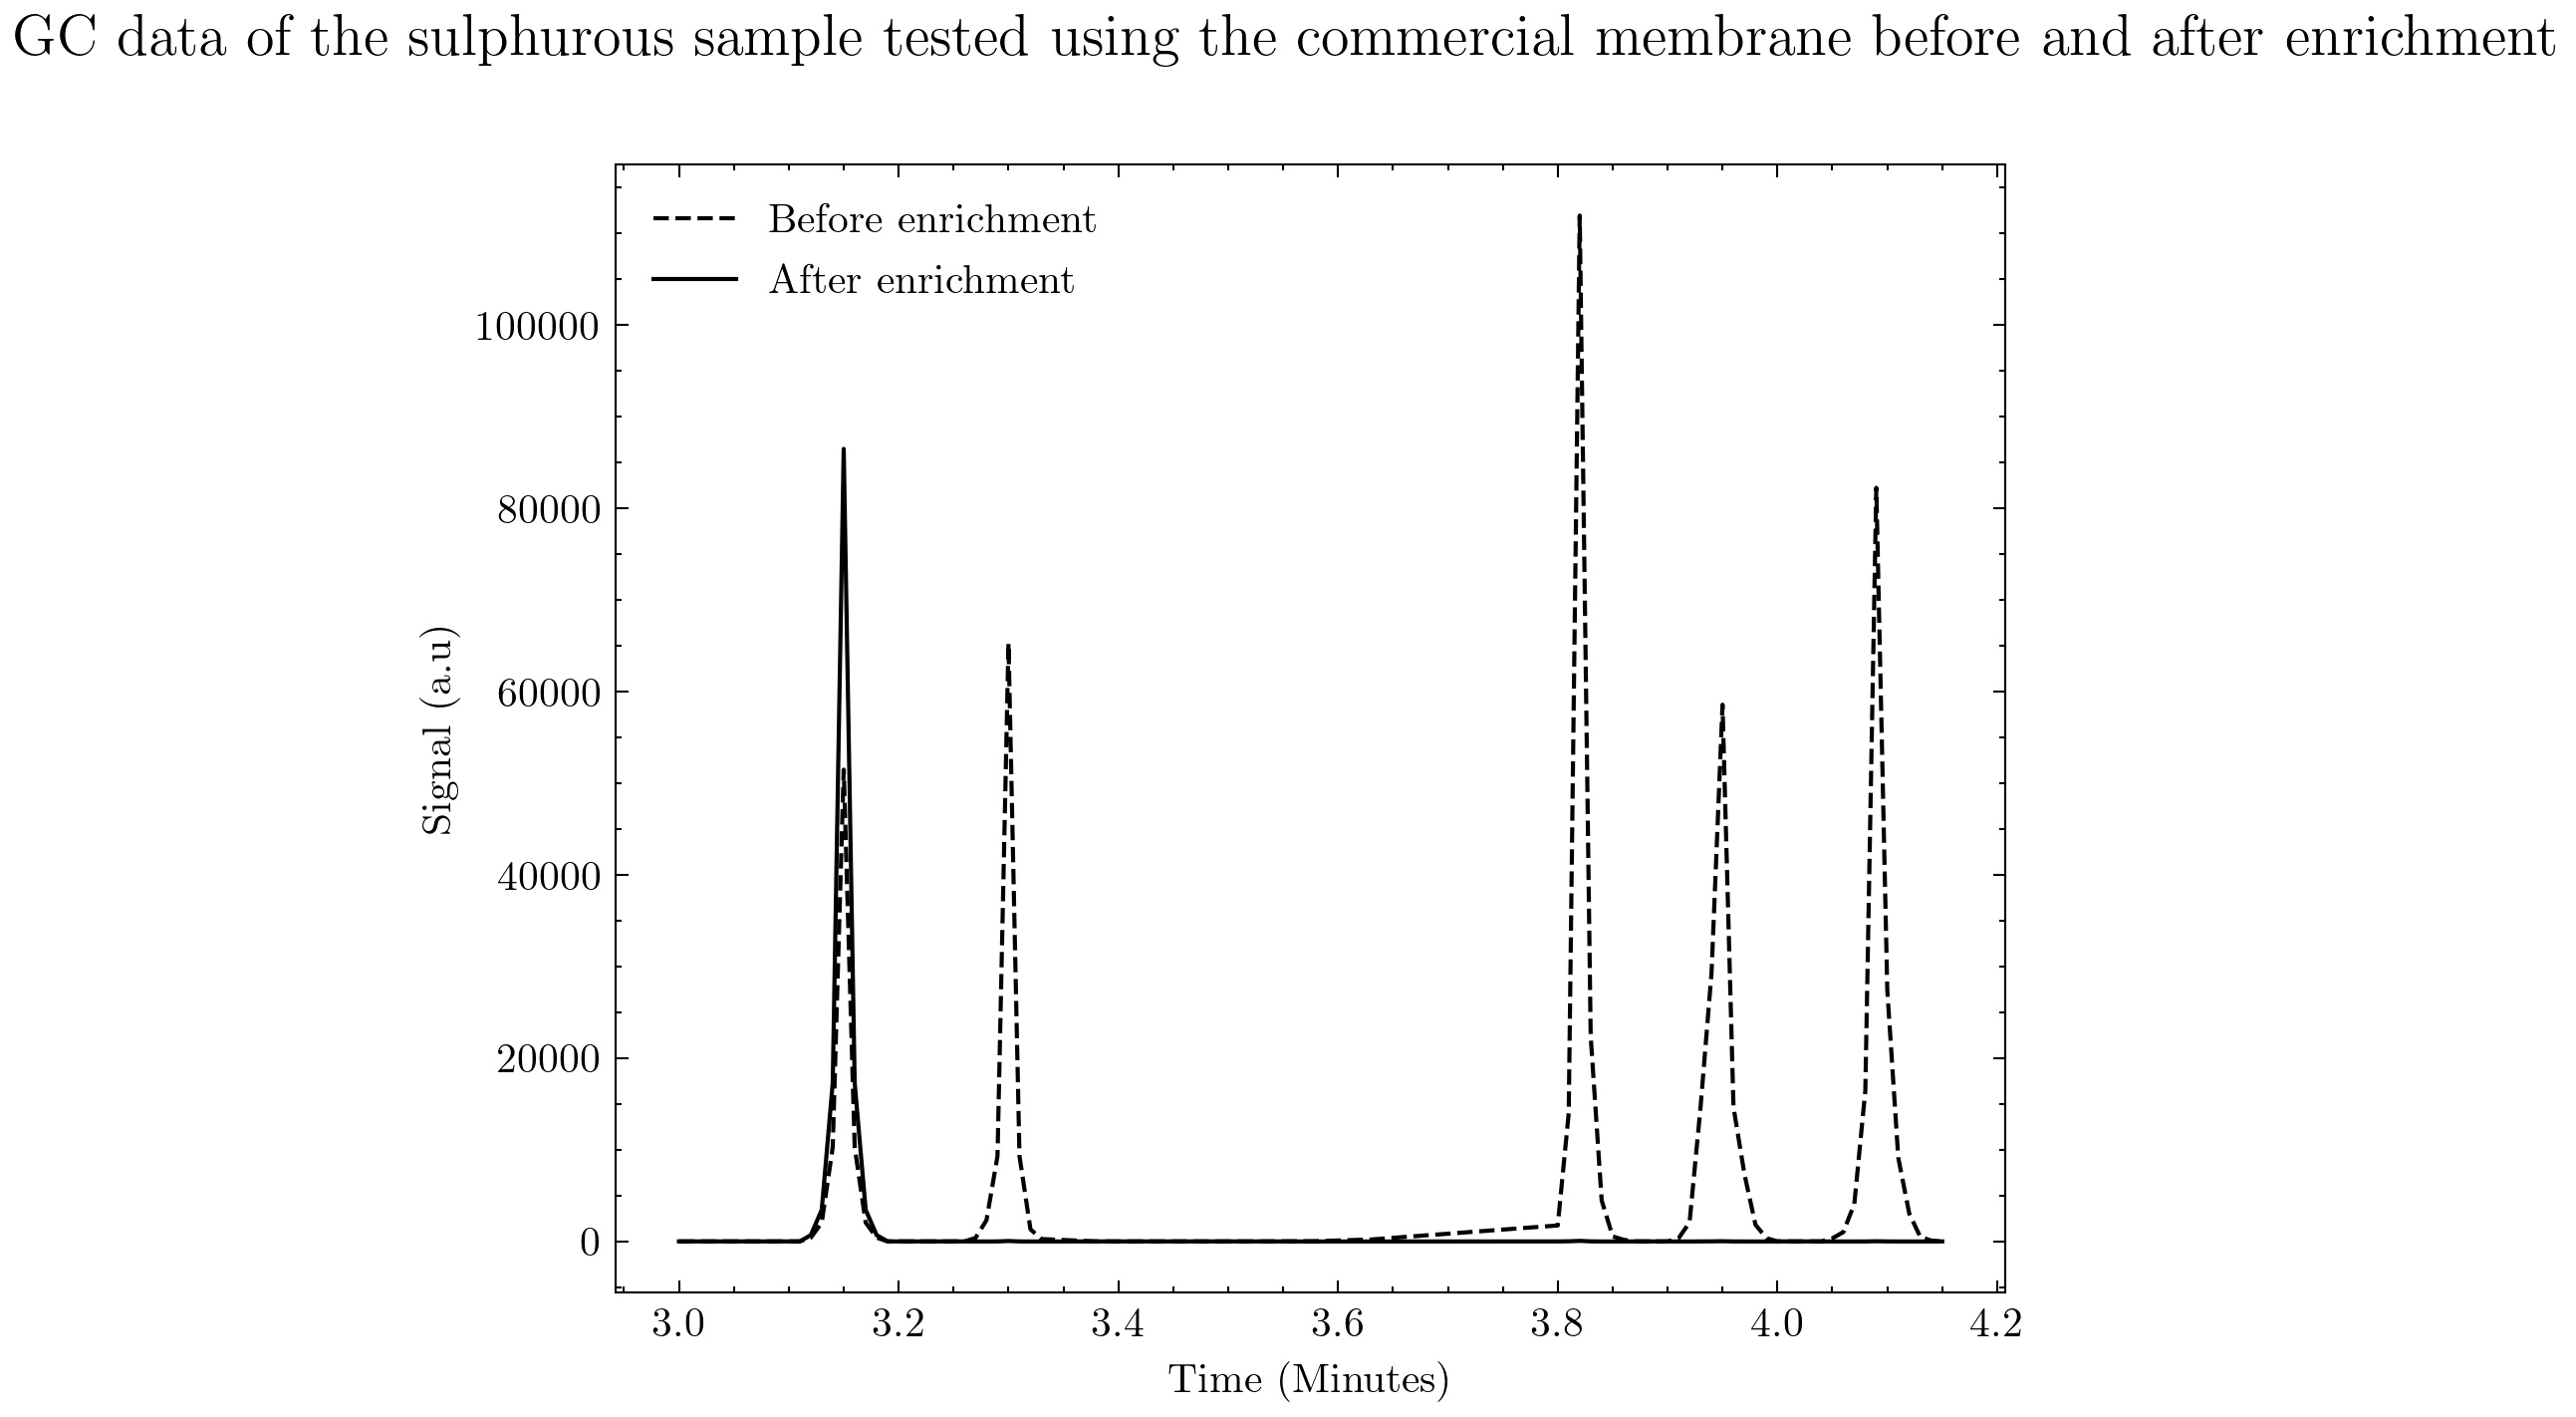
\includegraphics[width=\linewidth, keepaspectratio]{/Users/marc/Thesis/Chapter5/sulfcomgc.jpg}
    \caption{GC-PDHID data of the sulphurous sample both before and after enrichment with commercial membrane}
    \label{GCSULFCOMM}
\end{figure}

The PdCuZr membrane was tested twice, with both runs ending in failure due to delamination of the membrane after a number of temperature cycles. On the second attempt the heating ramp was lowered to 1 \textdegree C/min in order to put less thermal strain on the membrane. This resulted in the membrane lasting one extra temperature cycle, however made no lasting difference to the result. The reason for this is likely to be the combined force of the extra pressure in the enrichment vessel durting heating, and the multiple heating cooling cycles used over the course of the experiment causing the mismatch between the thermal expansion coefficient betwen the membrane and support to result in membrane failure. 

Since all enrichment experiments failed for the sulphur sample a comparison of the enrichment factors in sulphur containing atmospheres cannot be performed. 

\begin{landscape}
    \begin{figure}
        \centering
        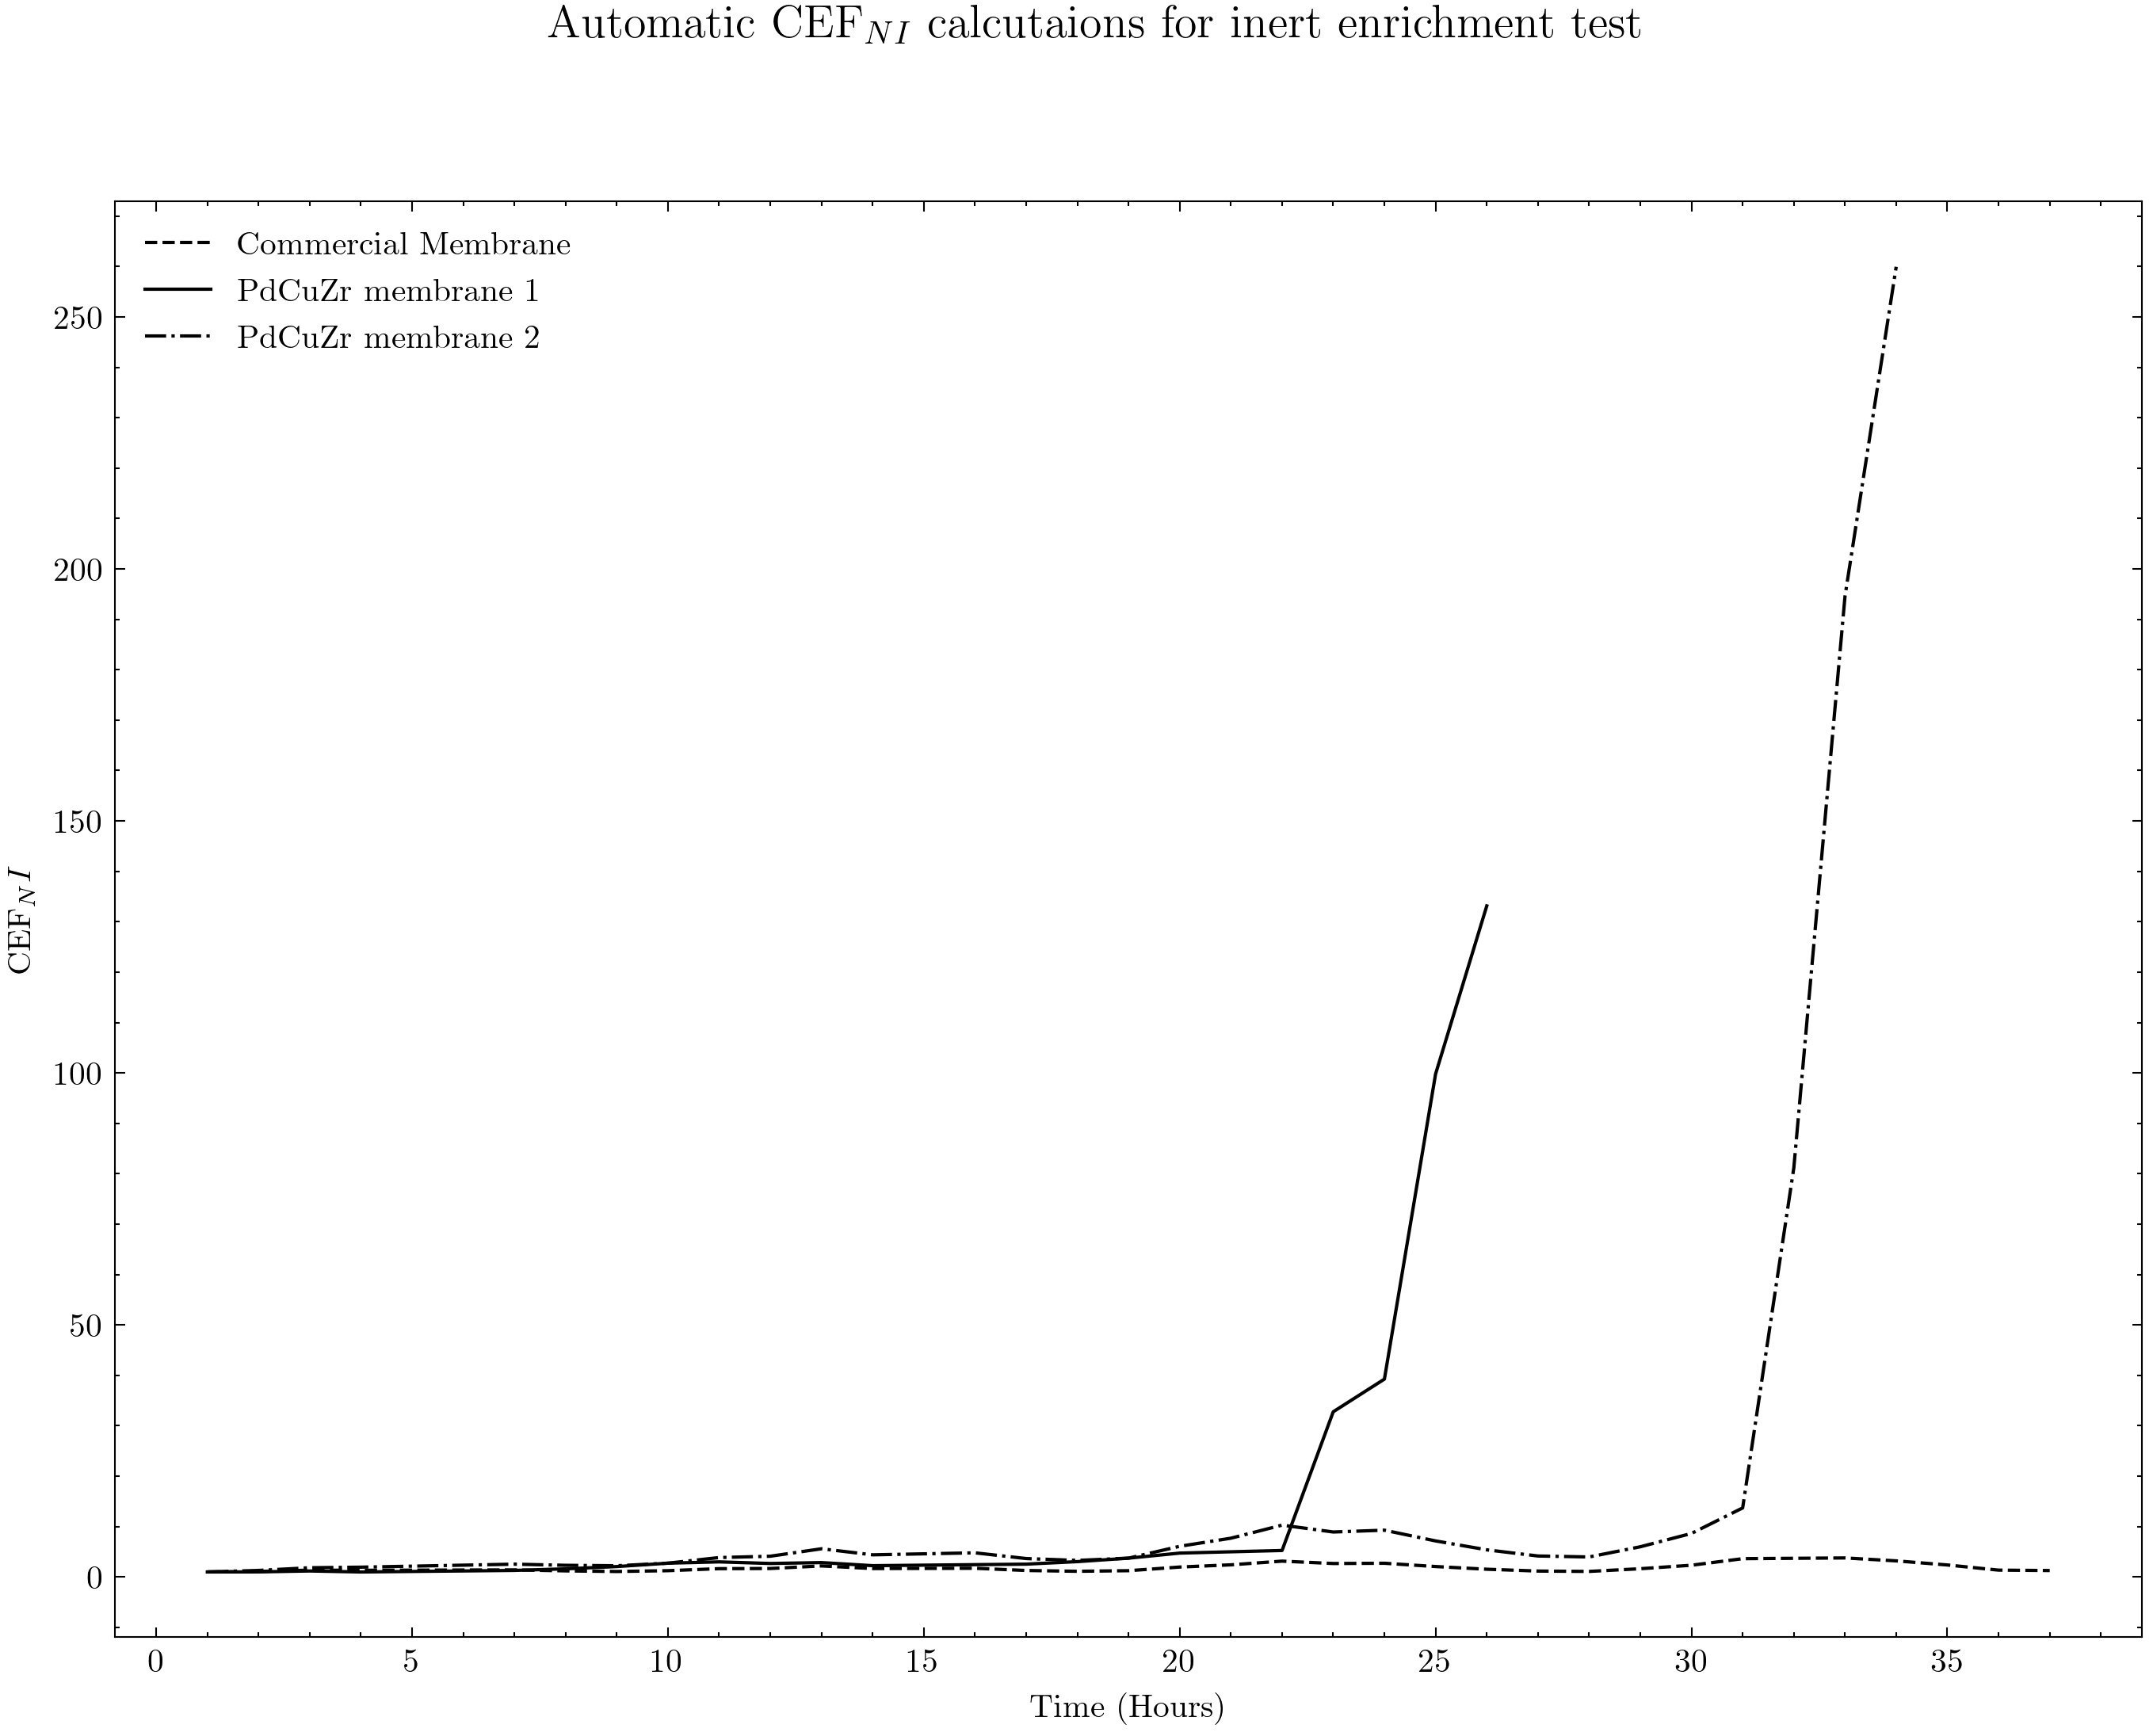
\includegraphics[width=0.9\linewidth, keepaspectratio]{/Users/marc/Thesis/Chapter5/sulfenrichni.jpg}
        \caption{$CEF_{NI}$ over the 40 hour enrichment of the sulphurous hydrogen sample shown in table \ref{exp-sulf}}
        \label{GCSULF}
    \end{figure}
\end{landscape}

\subsection{HRS sample}
The sample taken from the hydrogen refuelling station spiked with krypton as described in \ref{kryptonspike} was enriched using the commercial PdAuAG membrane as this was the only composition able to withstand the conditions required for enrichment. The enrichment was performed over 120 hours. Initial analysis showed that the krypton concentration in the sample before enrichment was 80 \textmu mol/mol and that nitrogen was present in the sample likely due to dead volume within the H\textsubscript{2} qualitizer. The CEF\textsubscript{NI} over the course of the experiment is shown in figure xx.

The sample was enriched to an enrichment factor of 41.76 as shown by the increase of krypton asnd nitrogen concentrations shown in figure xx. These peaks corresponded to concentrations of 3374 \textmu mol/mol of krypton and 957 \textmu mol/mol of Nitrogen respectivley. Using the tracer enrichment factor this corresponds to an initial concentration  of 22.91 \textmu mol/mol of Nitrogen  in the hydrogen sample. The results in the enriched sample also show a new peak at 2.4 minutes which corresponds to Argon, thereby proving that the method can be used to quantify impurities which were below the limit of detection of the detector in the initial sample. Due to the small size of the peak, quantifying the concentration was difficult and a higher enrichment factor would be required to accurately determine this. Unfortunately due to interrruptions from COVID-19 adequate time was not avaliable to perform this test. 

\section{Conclusion}
The enrichment device was successfully upgraded in order to improve it's reliability, safety, and the user interface for performing enrichment. This was done by changing the temperature controller to a PID control system which reduced the standard deviation of the temperature while at setpoint to 1.78\textdegree C. The safety and ergonomics of the device were improved by spliotting the device into two sections, the stationary unit, where majority of the piping, electronics, and safety interlocks are in place, and the transportable unit, which contained the enrichment vessel containing the membrane, and the gas to be analysed. 

The new enrichment device was tested using 3 hydrogen samples, a sample containing only inert impurities in order to test the device functions as required, a sulphur containing sample to test how the PdCuZr membrane identified as the best membrane in chapter \label{proc-testingchapref}, and a sample taken from a hydrogen refuelling station. The inert sample was successsfully enriched to 50x and using the tracer enrichment method using krypton the initial concentration of nitrogen was calculated to within 2\% of it's original value. 

The sulphur tests resulted in failure of all membranes used. For the commercial membrane this was due to high reactivity with the sulphur compounds which was also identified in chapter 5. For the PdCuZr membrane this was due to material instability and further work is required to manufacture the ceramic supported membrane to be ableto withstand temperature cycling. 

For the first time enrichment was performed on a real sample from a hydrogen refuelling station, proving both that the method is viable for analysis of real world hydrogen samples, and the protocol for spiking a hydrogen sample with krypton gas is approptiate. The sample was enriched 41 times and was able to accurately determine that the concentration of nitrogen in the sample before enrichment was 22.91 \textmu mol/mol. Enrichment also revealed the presence of Argon in the sample, which would not have been present in the analysis otherwise, further proving that the technique can provide a more accurate composition analysis of fuel grade hydrogen, past what is possible with commercial analysers.

\bibliographystyle{unsrtnat}
\bibliography{library.bib}